\documentclass[11pt,a4paper]{article}
% Editable source: compile with `sh build.sh` from this directory.
% Values and figures come from the executed Task 2 notebooks.
\usepackage[margin=21mm,headheight=16pt,headsep=8mm,footskip=12mm]{geometry}
\usepackage{fontspec}
\setmainfont{PT Serif}
\setsansfont{PT Sans}
\setmonofont{Menlo}[Scale=0.85]
\usepackage{polyglossia}
\setdefaultlanguage{ukrainian}
\setotherlanguage{english}
\newfontfamily\cyrillicfont{PT Serif}
\newfontfamily\cyrillicfontsf{PT Sans}
\newfontfamily\cyrillicfonttt{Menlo}[Scale=0.85]
\usepackage{amsmath,amssymb}
\usepackage{graphicx,float,booktabs,longtable,array}
\usepackage{xcolor}
\definecolor{accent}{HTML}{244A64}

% The editable Python sources live in code/. build.sh highlights them with Pygments.
\usepackage{fvextra}
\usepackage[most]{tcolorbox}
\input{build/code/style.tex}
\definecolor{answergreen}{HTML}{285C48}
\newtcolorbox{taskstatement}{enhanced,breakable,
  colback=accent!4!white,colframe=accent!35!white,colbacktitle=accent!10!white,
  coltitle=accent,fonttitle=\bfseries,title=Умова завдання,
  boxrule=0.4pt,arc=1mm,left=3mm,right=3mm,top=2mm,bottom=2mm,
  before skip=6pt,after skip=8pt}
\RecustomVerbatimEnvironment{Verbatim}{Verbatim}{
  fontsize=\fontsize{8.5}{10.5}\selectfont,breaklines=true,breakanywhere=true,
  breaksymbolleft={},breaksymbolright={},numbers=left,numbersep=6pt,xleftmargin=4mm}
\renewcommand{\theFancyVerbLine}{\sffamily\scriptsize\color{gray}\arabic{FancyVerbLine}}
\newcommand{\pythoncode}[1]{%
  \Needspace{6\baselineskip}
  \begin{tcolorbox}[enhanced,breakable,colback=black!2!white,colframe=black!15!white,
    colbacktitle=black!6!white,coltitle=accent,fonttitle=\bfseries\small,
    title=Код Python,title after break={Код Python (продовження)},boxrule=0.4pt,arc=1mm,left=2mm,right=2mm,top=2mm,bottom=2mm,
    before skip=6pt,after skip=8pt]
  \input{build/code/#1.tex}
  \end{tcolorbox}}
\newcommand{\answerheading}{\Needspace{4\baselineskip}\par\medskip
  {\color{answergreen}\bfseries Результати та інтерпретація}\par\smallskip}

\usepackage{titlesec}
\usepackage{needspace}
\pretocmd{\subsection}{\Needspace{8\baselineskip}}{}{}
\titleformat{\section}{\Large\bfseries\color{accent}}{Частина \thesection.}{0.5em}{}
\titleformat{\subsection}{\large\bfseries}{\thesubsection}{0.5em}{}
\usepackage{fancyhdr}
\pagestyle{fancy}
\fancyhf{}
\fancyhead[L]{\small Statistics and Econometrics}
\fancyhead[R]{\small\nouppercase{\leftmark}}
\fancyfoot[C]{\thepage}
\renewcommand{\sectionmark}[1]{\markboth{Частина \thesection}{}}
\renewcommand{\headrulewidth}{0.3pt}
\usepackage{caption}
\captionsetup{font=small,labelfont=bf}
\usepackage{hyperref}
\hypersetup{unicode=true,colorlinks=true,linkcolor=accent,urlcolor=accent,
  pdftitle={Завдання 2. Інференційна статистика},pdfauthor={Владислав Григола}}
\setlength{\parindent}{0pt}
\setlength{\parskip}{0.4em}
\setlength{\emergencystretch}{2em}
\linespread{1.02}
\raggedbottom
\providecommand{\tightlist}{\setlength{\itemsep}{0pt}\setlength{\parskip}{0pt}}
\begin{document}
\hypersetup{pageanchor=false}
\begin{titlepage}
\centering
\vspace*{14mm}
{\Large Український католицький університет\par}
\vspace{9mm}
{\large Statistics and Econometrics\par}
\vfill
{\huge\bfseries\color{accent} Завдання 2.\par}
\vspace{4mm}
{\huge\bfseries\color{accent} Інференційна статистика\par}
\vspace{10mm}
{\large Аналітичний звіт\par}
\vfill
{\large Виконав: \textbf{Владислав Григола}\par}
\vspace{22mm}
{\large 2026\par}
\end{titlepage}
\pagenumbering{arabic}
\hypersetup{pageanchor=true}
\markboth{Зміст}{}
\tableofcontents
\vspace{10mm}
\textbf{Дані та домовленості.}
У звіті виконано всі п’ять частин наданого завдання.
У самому файлі умова має заголовок «Задача 4»; цей звіт оформлено як навчальне Завдання 2.
Для частин 2 і 3 використано наданий \texttt{app\_metrics.csv}: 250 спостережень без пропусків.
Дані не змінювалися. Рівень значущості дорівнює $\alpha=0.05$; для частини 5 це явно прийнята домовленість.
В основних симуляціях використано початкове значення генератора 42;
для додаткової контрольної перевірки \textemdash{} 20261014.
Вибіркові дисперсії обчислено з дільником $n-1$.

Час у частині 1 вимірюється в умовних одиницях, оскільки одиницю в умові не вказано;
Session\_Time у частині 3 вимірюється у хвилинах. Валюту Revenue та Purchase\_Amount не задано.
Крапка використовується як десятковий роздільник. Наведені числові результати округлено;
розрахунки виконано з повною машинною точністю.
Кожен підпункт містить окремо умову, код Python та результати з інтерпретацією. Умови подано зі збереженням вимог і нумерації оригіналу. Код наведено з виконаних ноутбуків; кольором виділено ключові слова, рядки, числа та коментарі. Повні ноутбуки зі збереженими результатами підготовлено для індивідуального захисту.

\clearpage

\section*{Спільне налаштування Python}
\markboth{Налаштування}{}
Цей блок виконується на початку кожного ноутбука в окремому чистому ядрі.
Він імпортує бібліотеки, знаходить каталог завдання, створює каталоги результатів
та ініціалізує генератор випадкових чисел. Наступні блоки всередині кожної частини
виконуються послідовно. Команда \texttt{display} доступна в середовищі Jupyter.
\pythoncode{part1-cell1}
\clearpage
\section{Закон великих чисел, довірчі інтервали та ЦГТ}
\subsection*{Підготовка частини 1}
Задаємо параметри Gamma-розподілу, обсяги вибірок та кількість повторень.
\pythoncode{part1-cell2}
\subsection*{1(а). Вибіркові моменти та закон великих чисел}
\begin{taskstatement}
Нехай час між сесіями має Gamma-розподіл із параметрами форми $k=2$ і масштабу $\theta=5$, тому $\mu=10$, $\sigma^2=50$.
Змоделюйте вибірки розміром $n=5^1,5^2,\ldots,5^8$. Для кожної обчисліть вибіркове середнє та вибіркову дисперсію.
Побудуйте графік вибіркових середніх як функцію від $n$ з логарифмічною шкалою осі $X$.
Поясніть результат за допомогою слабкого закону великих чисел.
\end{taskstatement}


\pythoncode{part1-cell4}
\answerheading
Використано незалежні, а не вкладені вибірки: для кожного \(n=5^1,\ldots,5^8\) генерується нова вибірка. Параметр \(\theta=5\) є масштабом. Тому \[\mu=k\theta=10,\qquad \sigma^2=k\theta^2=50.\] Обчислено \[\bar X=\frac1n\sum_{i=1}^nX_i,\qquad s^2=\frac1{n-1}\sum_{i=1}^n(X_i-\bar X)^2.\] При \(n=5\) отримано \(\bar x=11.4887\), а при \(n=390625\) маємо \(\bar x=9.9963\) та \(s^2=49.7777\). Великі вибірки дають середні, близькі до 10. За слабким законом великих чисел для кожного \(\varepsilon>0\) маємо \(P(|\bar X_n-10|>\varepsilon)\to0\). Графік узгоджується з цим твердженням, але не доводить його. Збіжність не означає монотонного зменшення похибки в кожній реалізації. Для оцінки середнього часу між сесіями більша вибірка зазвичай дає точніший результат.

\begin{table}[H]
\centering
\small
\caption{Вибіркові моменти незалежних вибірок із розподілу Gamma(2, 5).}
\begin{tabular}{rrr}
\toprule
$n$ & $\bar x$ & $s^2$ \\
\midrule
5 & 11.488704 & 9.876565 \\
25 & 8.890425 & 21.964613 \\
125 & 10.097676 & 63.121252 \\
625 & 9.831200 & 45.690043 \\
3125 & 10.120737 & 49.760696 \\
15625 & 10.057645 & 51.695993 \\
78125 & 9.996694 & 50.433119 \\
390625 & 9.996343 & 49.777707 \\
\bottomrule
\end{tabular}
\end{table}

\begin{figure}[H]
\centering
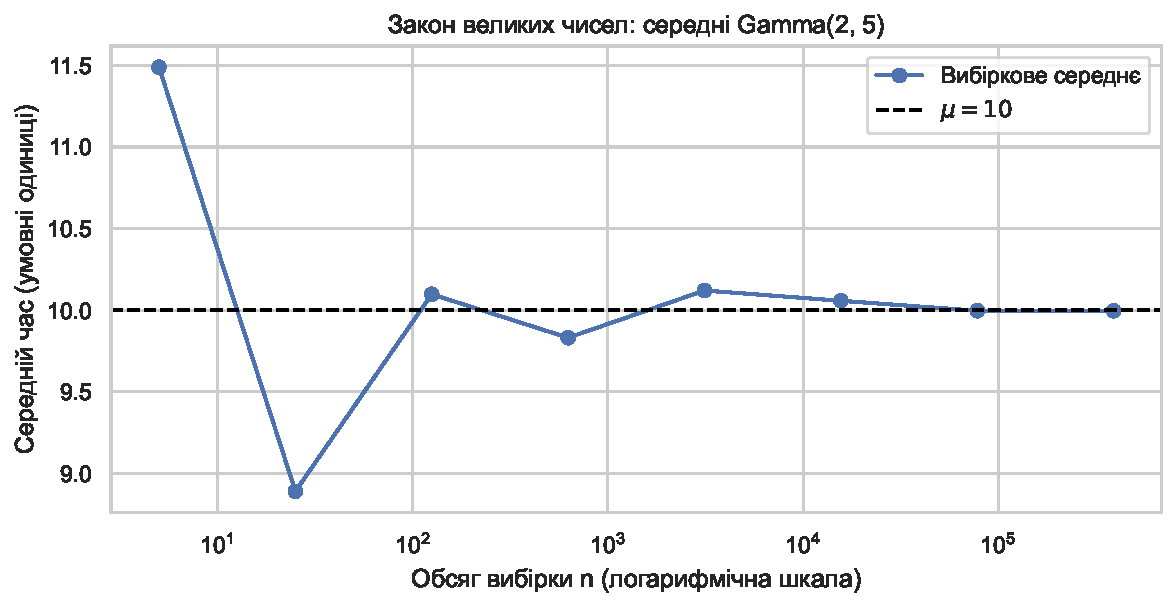
\includegraphics[width=0.90\linewidth]{../figures/part1_lln.pdf}
\caption{Траєкторія вибіркових середніх; вісь обсягу вибірки логарифмічна.}
\end{figure}
\subsection*{1(б). Довірчі інтервали для середнього}
\begin{taskstatement}
Для кожної вибірки вручну обчисліть 95\% довірчий інтервал для середнього $\mu$ і додайте його на графік.
Зробіть це двічі: з відомим теоретичним стандартним відхиленням $\sigma$ та з оціненим вибірковим стандартним відхиленням $s$.
Обговоріть спостереження та теоретично поясніть результати при малих і великих $n$.
\end{taskstatement}


\pythoncode{part1-cell7}
\answerheading
Інтервали побудовано за формулами \[I_\sigma=\left[\bar x-z_{0.975}\frac{\sqrt{50}}{\sqrt n},\ \bar x+z_{0.975}\frac{\sqrt{50}}{\sqrt n}\right],\qquad z_{0.975}\approx1.9600,\] \[I_s=\left[\bar x-t_{0.975,n-1}\frac{s}{\sqrt n},\ \bar x+t_{0.975,n-1}\frac{s}{\sqrt n}\right].\] Другий інтервал використовує оцінене стандартне відхилення та квантиль Стьюдента. Обидва інтервали тут \textbf{наближені}: Gamma-дані не є нормальними, а точний t-інтервал вимагає нормальності генеральної сукупності. При малих \(n\) фактичне покриття може відрізнятися від 95\%.

Для \(n=5\) отримано \(I_\sigma=[5.2908;\ 17.6867]\) та \(I_s=[7.5865;\ 15.3909]\). У цій вибірці \(s^2=9.8766\) значно менша за 50, тому інтервал з оціненим \(s\) вужчий, попри більший t-квантиль. Він не зобов'язаний завжди бути ширшим. При великих \(n\) маємо \(s\to\sigma\), t-квантиль наближається до z-квантиля, а ЦГТ покращує нормальне наближення. Ширина інтервалів зменшується приблизно як \(1/\sqrt n\).

У цій реалізації всі інтервали містять 10. Вісім інтервалів не є оцінкою довгострокового 95\% покриття. Рівень 95\% характеризує частку інтервалів, які накривали б фіксоване \(\mu\) при багаторазовому повторенні процедури за відповідних умов.

\begin{table}[H]
\centering
\small
\caption{Наближені 95\% довірчі інтервали.}
\begin{tabular}{rcc}
\toprule
$n$ & $I_\sigma$ & $I_s$ \\
\midrule
5 & [5.2908; 17.6867] & [7.5865; 15.3909] \\
25 & [6.1186; 11.6622] & [6.9559; 10.8250] \\
125 & [8.8581; 11.3373] & [8.6912; 11.5042] \\
625 & [9.2768; 10.3856] & [9.3002; 10.3622] \\
3125 & [9.8728; 10.3687] & [9.8733; 10.3682] \\
15625 & [9.9468; 10.1685] & [9.9449; 10.1704] \\
78125 & [9.9471; 10.0463] & [9.9469; 10.0465] \\
390625 & [9.9742; 10.0185] & [9.9742; 10.0185] \\
\bottomrule
\end{tabular}
\end{table}

\begin{figure}[H]
\centering
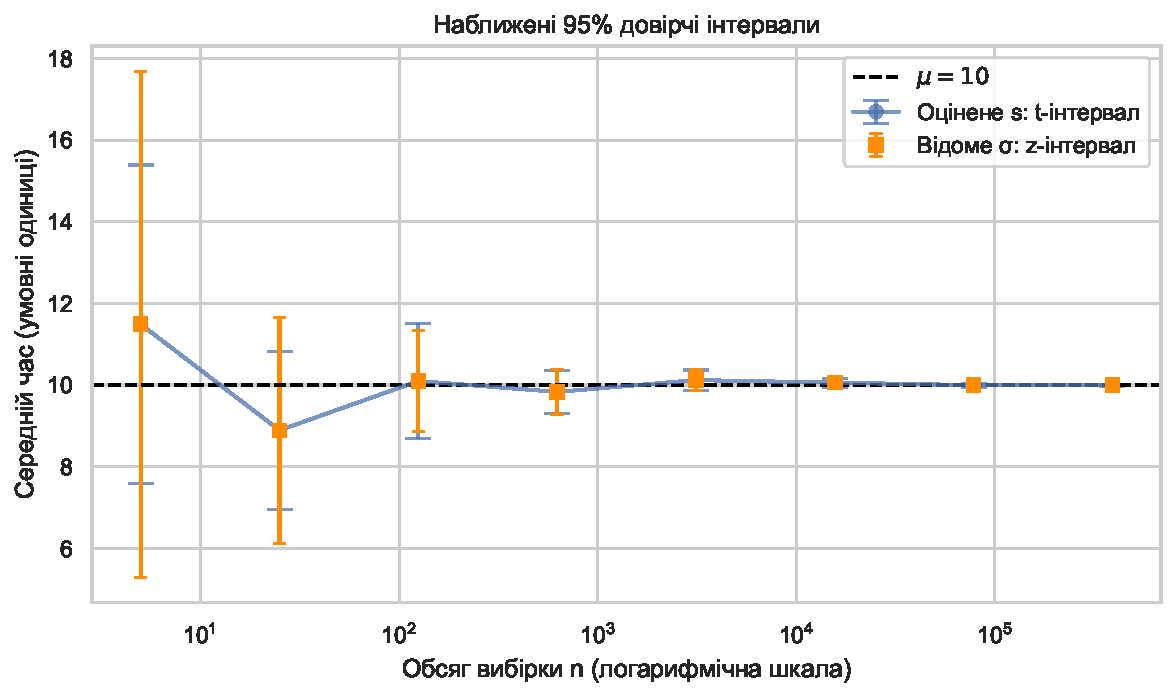
\includegraphics[width=0.80\linewidth]{../figures/part1_intervals.pdf}
\caption{Інтервали з відомим та оціненим стандартним відхиленням.}
\end{figure}
\subsection*{1(в). Розподіли середніх і дисперсій при обсязі 4}
\begin{taskstatement}
Змоделюйте $b=1000$ вибірок обсягу $n=4$ з асиметричного розподілу $\Gamma(2,5)$.
Для кожної оцініть і збережіть середнє та дисперсію. Побудуйте гістограму 1000 вибіркових середніх і гістограму 1000 вибіркових дисперсій.
\end{taskstatement}


\pythoncode{part1-cell10}
\answerheading
Згенеровано 1000 незалежних вибірок обсягу 4. Для кожної збережено \(\bar x\) та незміщену дисперсію \(s^2\) з дільником \(n-1=3\). Середнє 1000 оцінок \(\bar x\) дорівнює 10.1350, а середнє 1000 оцінок \(s^2\) становить 50.9810. Вони близькі до 10 і 50 відповідно. Обидві гістограми мають праву асиметрію; дисперсії особливо нестійкі для такої малої вибірки. Окремі великі значення збільшують правий хвіст гістограми дисперсій.

\begin{figure}[H]
\centering
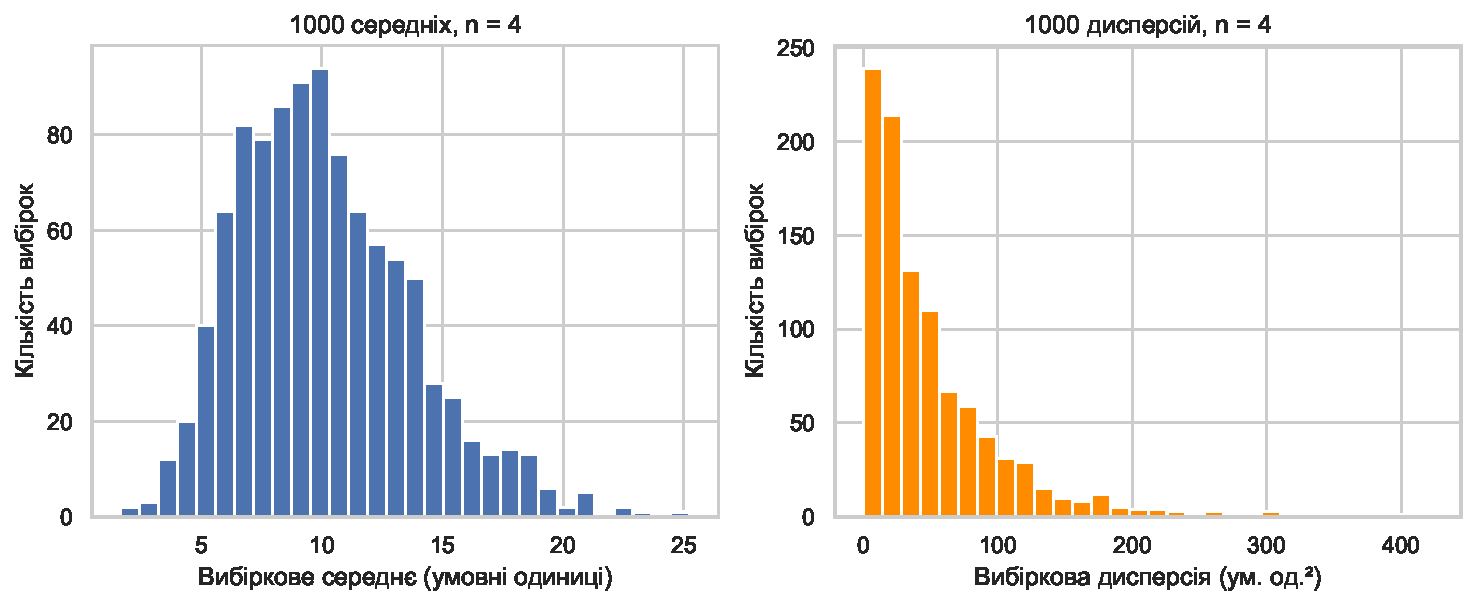
\includegraphics[width=\linewidth]{../figures/part1_histograms.pdf}
\caption{Гістограми 1000 середніх та 1000 незміщених вибіркових дисперсій.}
\end{figure}
\subsection*{1(г). Аналітичні моменти вибіркового середнього}
\begin{taskstatement}
Використовуючи властивості розподілу, обраного в пункті 1(в), аналітично обчисліть
\[
E\!\left(\frac{X_1+X_2+X_3+X_4}{4}\right),\qquad
\operatorname{Var}\!\left(\frac{X_1+X_2+X_3+X_4}{4}\right).
\]
\end{taskstatement}


\pythoncode{part1-cell13}
\answerheading
Нехай \(X_1,\ldots,X_4\) незалежні й однаково розподілені як \(\Gamma(2,5)\). За лінійністю сподівання \[E(\bar X)=\frac14\sum_{i=1}^4E(X_i)=\frac{4\cdot10}{4}=10.\] Незалежність дає нульові коваріації, тому \[\operatorname{Var}(\bar X)=\frac1{16}\sum_{i=1}^4\operatorname{Var}(X_i)=\frac{4\cdot50}{16}=12.5.\] Звідси стандартне відхилення середнього дорівнює \(\sqrt{12.5}\approx3.5355\). Емпірична дисперсія 1000 середніх становить 13.0804, що близько до 12.5. Незалежність потрібна саме для використаної формули дисперсії.
\subsection*{1(д). Нормальне наближення та центральна гранична теорема}
\begin{taskstatement}
До гістограми середніх додайте теоретичну нормальну щільність із математичним сподіванням і дисперсією, знайденими в пункті 1(г).
Порівняйте щільність із гістограмою. Поясніть, якого результату очікуєте і чому.
Що зміниться, якщо збільшити обсяг кожної вибірки з 4 до 100? Обґрунтуйте відповідь за допомогою центральної граничної теореми.
\end{taskstatement}
\textbf{Прогноз перед моделюванням.}

Перед побудовою графіка очікую, що при \(n=4\) нормальна щільність лише приблизно описуватиме середні: асиметрія ще помітна. При \(n=100\) за ЦГТ наближення має бути кращим, а дисперсія середнього зменшиться з \(50/4\) до \(50/100\).

\pythoncode{part1-cell16}
\clearpage
\answerheading
\begin{figure}[H]
\centering
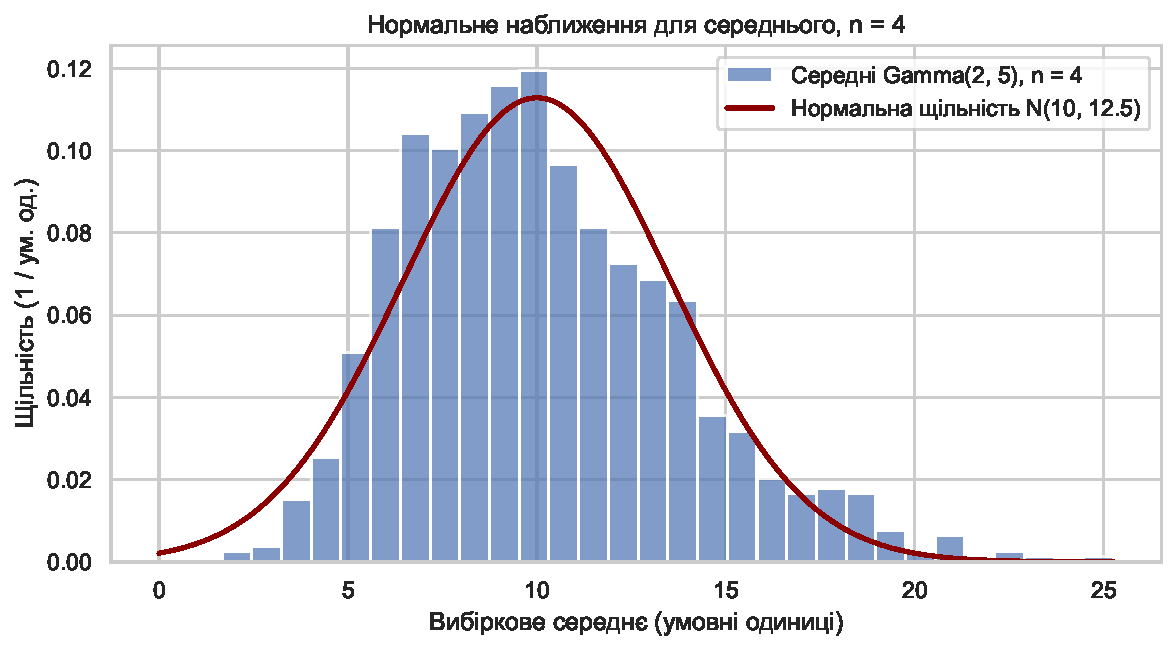
\includegraphics[width=0.90\linewidth]{../figures/part1_normal_approximation.pdf}
\caption{Порівняння щільності середніх при обсязі 4 з нормальним наближенням.}
\end{figure}
На гістограму щільності накладено нормальну щільність \(N(10,12.5)\), де другий параметр позначає дисперсію. Її центр і масштаб близькі до емпіричних, однак гістограма при \(n=4\) залишається асиметричною; симетрична нормальна крива не відтворює правий хвіст і навіть допускає від'ємні середні. Це узгоджується з прогнозом перед побудовою графіка.

За ЦГТ для незалежних однаково розподілених величин зі скінченними сподіванням і дисперсією \[\frac{\sqrt n(\bar X_n-10)}{\sqrt{50}}\ \xrightarrow{d}\ N(0,1).\] При \(n=100\) очікуємо краще наближення \(\bar X_{100}\approx N(10,0.5)\): середнє залишається 10, а дисперсія дорівнює \(50/100=0.5\). Саме збільшення обсягу кожної вибірки покращує нормальне наближення. Збільшення кількості повторень при незмінному \(n=4\) лише точніше показало б той самий ненормальний розподіл середнього.

\clearpage
\section{Оцінювання максимальною правдоподібністю}
\subsection*{Підготовка частини 2}
Завантажуємо наданий CSV, перевіряємо потрібні колонки, бінарні значення та пропуски.
\pythoncode{part2-cell2}
\subsection*{2(а). Перевірка нормальності реєстрацій}
\begin{taskstatement}
Завантажте колонку \texttt{Registration\_Success} із \texttt{app\_metrics.csv}.
Виконайте одновибірковий критерій Колмогорова--Смирнова в модифікації Лілієфорса, коли параметри розподілу невідомі й оцінюються за вибіркою.
Перевірте можливість нормального наближення цих бінарних даних. Запишіть $H_0$, $H_1$, статистику, p-значення та висновок.
\end{taskstatement}


\pythoncode{part2-cell4}
\answerheading
У файлі 250 спостережень без пропусків; успішних реєстрацій 68. Припускаємо незалежність користувачів. За вимогою завдання перевіряємо \(H_0\): розподіл спостережень нормальний з невідомими параметрами; \(H_1\): він не є нормальним. Рівень значущості \(\alpha=0.05\).

Виклик \texttt{lilliefors(registrations,\ dist="norm",\ pvalmethod="table")} повернув \(D=0.457078\) та \(p_{\mathrm{returned}}=0.001\). Це нижня межа табличної реалізації statsmodels: коректно записувати \(p\le0.001\), а не вважати 0.001 точним p-значенням. Формально тест відхиляє \(H_0\).

Водночас бінарна величина має лише значення 0 і 1, тому не може мати неперервний нормальний розподіл. Тест Лілієфорса розрахований на неперервні дані, тому для бінарних значень 0 і 1 його p-значення може бути неточним. Для окремої реєстрації використовуємо розподіл Бернуллі. Нормальне наближення може стосуватися вибіркової частки при великому обсязі, а не окремих нулів та одиниць.
\subsection*{2(б). Правдоподібність Бернуллі та чисельна оцінка}
\begin{taskstatement}
Запишіть функцію правдоподібності $L(p)$ і логарифмічну функцію $\ln L(p)$ для вибірки Бернуллі.
Реалізуйте від’ємну логарифмічну правдоподібність
\[
-\ln L(p)=-\sum_{t=1}^{T}\bigl(r_t\ln p+(1-r_t)\ln(1-p)\bigr).
\]
Знайдіть оптимальну оцінку за допомогою \texttt{scipy.optimize.minimize} з обмеженням $p\in[10^{-5},1-10^{-5}]$.
Порівняйте чисельну оцінку $\widehat p_{MLE}$ з вибірковим середнім.
У вихідній умові після формули NLL вжито слово «максимізуйте»; напрям оптимізації пояснено у відповіді.
\end{taskstatement}


\pythoncode{part2-cell7}
\answerheading
Нехай \(r_t\in\{0,1\}\), \(T=250\), \(S=\sum_{t=1}^T r_t=68\). Для незалежних випробувань зі спільною ймовірністю \(p\): \[L(p)=\prod_{t=1}^{T}p^{r_t}(1-p)^{1-r_t}=p^{68}(1-p)^{182},\] \[\ell(p)=\ln L(p)=68\ln p+182\ln(1-p),\qquad \operatorname{NLL}(p)=-\ell(p).\] Максимізація \(\ell(p)\) еквівалентна \textbf{мінімізації} NLL; слово «максимізуйте» після від'ємного логарифма в умові є неточністю. Аналітично \[\ell'(p)=\frac{68}{p}-\frac{182}{1-p}=0\quad\Longrightarrow\quad\widehat p=\frac{68}{250}=0.272.\] Друга похідна \(\ell''(p)=-68/p^2-182/(1-p)^2<0\), тому це максимум. Чисельний мінімум \texttt{scipy.optimize.minimize} на \([10^{-5},1-10^{-5}]\) дає \(\widehat p_{MLE}=0.27199997\); вибіркове середнє дорівнює 0.272. Абсолютна різниця \(3.2544\times 10^{-8}\) зумовлена чисельною похибкою оптимізації. Оцінена конверсія становить 27.2\%.
\subsection*{2(в). Ймовірності кількості майбутніх реєстрацій}
\begin{taskstatement}
За знайденою оцінкою $\widehat p$ обчисліть імовірності для наступних 20 відвідувачів:
\begin{itemize}
\item зареєструються рівно 5;
\item зареєструються щонайменше 8;
\item кількість реєстрацій буде строго більшою за $20\widehat p$.
\end{itemize}
Використайте PMF та CDF біноміального розподілу.
\end{taskstatement}


\pythoncode{part2-cell10}
\answerheading
За припущення незалежності майбутніх відвідувачів і незмінної ймовірності реєстрації \(K\sim\operatorname{Bin}(20,\widehat p)\). Використовуємо знайдену чисельну оцінку \(\widehat p\): \[P(K=5)=\binom{20}{5}\widehat p^5(1-\widehat p)^{15}=0.197360,\] \[P(K\ge8)=1-F_K(7)=0.150328.\] Оскільки \(E(K)=20\widehat p\approx5.44\), строго більше за сподівання означає щонайменше 6 реєстрацій: \[P(K>20\widehat p)=P(K\ge6)=1-F_K(5)=0.472429.\] Ймовірності обчислено функціями \texttt{binom.pmf} та \texttt{binom.sf} (остання дорівнює \(1-\mathrm{CDF}\)). Це модельний прогноз із підставленою оцінкою \(p\), який не враховує невизначеність самої оцінки та можливі зміни поведінки користувачів.

\clearpage
\section{Перевірка гіпотез про продуктові метрики}
\subsection*{Підготовка частини 3}
Завантажуємо наданий CSV, перевіряємо потрібні колонки, бінарні значення та пропуски.
\pythoncode{part3-cell2}
\subsection*{3(а). Чи перевищує середній час сесії 15 хвилин?}
\begin{taskstatement}
Продакт-менеджер стверджує, що очікуваний час утримання користувача \texttt{Session\_Time} перевищує 15 хвилин.
Перевірте це твердження відповідним одностороннім параметричним критерієм при $\alpha=0.05$.
Наведіть гіпотези, формулу статистики з числовою підстановкою, критичну область, p-значення, рішення та бізнес-висновок.
\end{taskstatement}


\pythoncode{part3-cell4}
\answerheading
\textbf{Гіпотези:} \(H_0:\mu\le15\) проти \(H_1:\mu>15\); статистику обчислюємо на межі \(\mu_0=15\). Дані містять \(n=250\) значень без пропусків. Припускаємо незалежну репрезентативну вибірку зі скінченною дисперсією. Точний t-критерій вимагає нормальності; при великому \(n\) використовуємо наближення для середнього.

\textbf{Статистика та критична область:} \[t=\frac{\bar x-15}{s/\sqrt n}=\frac{16.52012-15}{5.000818/\sqrt{250}}=4.806255,\qquad df=249.\] Відхиляємо \(H_0\), якщо \(t>t_{0.95,249}=1.650996\).

\textbf{Результат:} \(p=1.3306\times 10^{-6}<0.05\), тому \(H_0\) відхиляємо. Є статистичні підстави вважати, що середній час сесії перевищує 15 хвилин. У вибірці середній час дорівнює 16.52012 хв, тобто приблизно на 1.52 хв більше за поріг. Висновок стосується середнього, а не кожного користувача, і спирається на припущення щодо вибірки.
\subsection*{3(б). Порівняння Revenue між iOS та Android}
\begin{taskstatement}
Перевірте, чи відрізняється середній \texttt{Revenue} користувачів iOS від середнього \texttt{Revenue} користувачів Android.
Генеральні дисперсії невідомі та не обов’язково рівні: використайте двосторонній t-критерій Уелша при $\alpha=0.05$.
Наведіть гіпотези, формулу статистики з числовою підстановкою, критичну область, p-значення, рішення та бізнес-висновок.
\end{taskstatement}


\pythoncode{part3-cell7}
\answerheading
\textbf{Гіпотези:} \(H_0:\mu_I=\mu_A\), \(H_1:\mu_I\ne\mu_A\), де \(I\) позначає iOS, \(A\) - Android. Використано 110 та 140 спостережень відповідно, пропусків немає. Припускаємо незалежність користувачів і груп та скінченні дисперсії; рівності дисперсій не вимагаємо. Для ненормальних сукупностей висновок є наближеним; обидві групи досить великі для застосування ЦГТ за цих умов.

\textbf{Статистика Уелша:} \[t=\frac{\bar x_I-\bar x_A}{\sqrt{s_I^2/n_I+s_A^2/n_A}}
=\frac{500.9221-393.5084}{\sqrt{65010.5061/110+17623.7712/140}}=4.011751.\] Число ступенів свободи оцінено за формулою \[\nu=\frac{(s_I^2/n_I+s_A^2/n_A)^2}{(s_I^2/n_I)^2/(n_I-1)+(s_A^2/n_A)^2/(n_A-1)}=154.869447.\] Відхиляємо \(H_0\), якщо \(|t|>t_{0.975,\nu}=1.975400\).

\textbf{Результат:} \(p=9.3545\times 10^{-5}<0.05\), тому \(H_0\) відхиляємо. Дані свідчать про відмінність середнього Revenue між платформами. Середнє iOS вище приблизно на 107.41 грошових одиниць. Валюту в умові не вказано. Цей зв'язок не доводить, що саме платформа спричиняє різницю: групи можуть відрізнятися складом користувачів. Перевірка нормальності сукупного Revenue у пункті 3(д) не є окремою перевіркою нормальності кожної групи.
\subsection*{3(в). Лінійний зв’язок переглядів і суми покупки}
\begin{taskstatement}
Перевірте гіпотезу про відсутність зв’язку між кількістю переглядів \texttt{Page\_Views} і сумою покупки \texttt{Purchase\_Amount}
за допомогою критерію для коефіцієнта лінійної кореляції Пірсона при $\alpha=0.05$.
Наведіть гіпотези, формулу статистики з числовою підстановкою, критичну область, p-значення, рішення та бізнес-висновок.
\end{taskstatement}


\pythoncode{part3-cell10}
\answerheading
\textbf{Гіпотези:} \(H_0:\rho=0\), \(H_1:\rho\ne0\). Перевіряємо саме лінійний зв'язок. Використано 250 пар Page\_Views та Purchase\_Amount; пропусків немає. Якби вони були, вилучалися б цілі пари. Припускаємо незалежність пар. Звичайна формула p-значення спирається на спільний нормальний розподіл двох ознак. Page\_Views є кількістю переглядів, тому ця умова не виконується точно; p-значення використовуємо як наближення.

\textbf{Статистика:} \[r=\frac{\sum_i(x_i-\bar x)(y_i-\bar y)}{\sqrt{\sum_i(x_i-\bar x)^2\sum_i(y_i-\bar y)^2}}
=\frac{88681.7496}{\sqrt{1940.9640\cdot4948498.8700}}=0.904875,\] \[t=r\sqrt{\frac{n-2}{1-r^2}}=0.904875\sqrt{\frac{248}{1-0.904875^2}}=33.476102.\] За \(df=248\) критична область: \(|t|>t_{0.975,248}=1.969576\).

\textbf{Результат:} \(p=5.7422\times 10^{-94}<0.05\), тому за використаним критерієм \(H_0\) відхиляємо. Спостерігаємо сильний додатний лінійний зв'язок: користувачі з більшою кількістю переглядів зазвичай мають вищу суму покупки. Це не доводить причинного впливу переглядів на покупку. Нульова кореляція також не означала б загальної незалежності.
\subsection*{3(г). Чи перевищує частка підписок 10\%?}
\begin{taskstatement}
Перевірте, чи генеральна частка користувачів із платною підпискою \texttt{Subscription} статистично значущо перевищує 10\%.
Використайте $\alpha=0.05$. Наведіть гіпотези, формулу статистики з числовою підстановкою, критичну область, p-значення, рішення та бізнес-висновок.
\end{taskstatement}


\pythoncode{part3-cell13}
\answerheading
\textbf{Гіпотези:} \(H_0:p\le0.10\) проти \(H_1:p>0.10\). Маємо 250 бінарних спостережень без пропусків та 34 підписки, тому \(\widehat p=34/250=0.136\). Припускаємо незалежні випробування Бернуллі зі спільною ймовірністю успіху. Для нормального наближення на межі \(H_0\) перевіряємо \(np_0=25\) та \(n(1-p_0)=225\); обидва значення перевищують 10.

\textbf{Статистика:} \[z=\frac{\widehat p-p_0}{\sqrt{p_0(1-p_0)/n}}
=\frac{0.136-0.10}{\sqrt{0.10\cdot0.90/250}}=1.897367.\] У \texttt{proportions\_ztest} явно задано \texttt{prop\_var=0.10}, щоб використати дисперсію за \(H_0\). Критична область: \(z>z_{0.95}=1.644854\).

\textbf{Результат:} одностороннє \(p=0.028890<0.05\), тому \(H_0\) відхиляємо. Дані підтримують твердження, що генеральна частка платних підписок перевищує 10\%. Вибіркова частка дорівнює 13.6\%, тобто на 3.6 відсоткового пункту вище за поріг. Це наближений висновок за припущень тесту; нормально розподілені окремі бінарні спостереження не потрібні.
\clearpage
\subsection*{3(д). Перевірка нормальності Revenue}
\begin{taskstatement}
Перевірте нормальність метрики \texttt{Revenue} одновибірковим критерієм Колмогорова--Смирнова в модифікації Лілієфорса.
Використайте виключно вбудовану функцію \texttt{statsmodels}, без ручного обчислення статистики, при $\alpha=0.05$.
Наведіть гіпотези, отриману статистику, p-значення та висновок щодо припущень попередніх тестів.
\end{taskstatement}


\pythoncode{part3-cell16}
\answerheading
\textbf{Гіпотези:} \(H_0\): Revenue має нормальний розподіл з невідомими параметрами; \(H_1\): розподіл відрізняється від нормального. Використано 250 спостережень без пропусків; припускаємо незалежність і однаковий розподіл спостережень.

\textbf{Вбудована функція:} \texttt{lilliefors} із модуля \texttt{statsmodels.stats.diagnostic}.

Виклик: \texttt{lilliefors(revenue, dist="norm", pvalmethod="table")}.

Статистику вручну не обчислюємо, як вимагає цей підпункт. Отримано \(D=0.146746\) та \(p_{\mathrm{returned}}=0.001\). Це нижня таблична межа, тому записуємо \(p\le0.001\). Правило відхилення: \(p<0.05\).

\textbf{Результат:} нормальність сукупного Revenue відхиляємо. Просту нормальну модель розподілу індивідуального доходу ці дані не підтримують. Проте це не автоматично скасовує всі попередні висновки. Критерії для середніх можуть спиратися на ЦГТ при великих незалежних вибірках зі скінченною дисперсією; для Уелша важливі розподіли всередині платформ. Критерій Пірсона має окремі вимоги до спільного розподілу двох ознак. Критерій для частки використовує бінарні дані та нормальне наближення частки, а не нормальність окремих значень. Твердження умови про обов'язкову нормальність усіх ознак потребує цього уточнення.

Усі перевірки частини 3 виконано окремо при \(\alpha=0.05\), як задано. Спільний рівень помилки для всієї серії тестів не контролюється.

\clearpage
\section{Емпіричний рівень помилки першого роду}
\subsection*{Підготовка частини 4}
Після спільного блоку налаштування задаємо параметри експерименту.
\pythoncode{part4-cell2}
\subsection*{4(а). Двосторонній t-критерій для однієї вибірки}
\begin{taskstatement}
Змоделюйте вибірку обсягу $n=30$ із нормального розподілу з $\mu_0=100$ і $\sigma^2=25$.
Перевірте $H_0:\mu=100$ проти двосторонньої альтернативи, вважаючи генеральну дисперсію невідомою.
Вручну обчисліть тестову статистику, визначте аналітичну критичну область для $\alpha=0.05$ і прийміть рішення.
\end{taskstatement}


\pythoncode{part4-cell4}
\answerheading
Моделюємо \(X_i\sim N(100,25)\), тобто генератор використовує стандартне відхилення 5. У тесті дисперсію вважаємо невідомою. Гіпотези: \(H_0:\mu=100\), \(H_1:\mu\ne100\). \[t=\frac{\bar x-100}{s/\sqrt{30}}=\frac{100.084071-100}{3.883745/\sqrt{30}}=0.118564.\] За незалежності та нормальності при \(H_0\) маємо \(T\sim t_{29}\). Критична область рівня 0.05: \[(-\infty,-t_{0.975,29})\cup(t_{0.975,29},\infty),\qquad |t|>2.045230.\] Отримано \(p=0.906438\), тому \(H_0\) не відхиляємо. У цій вибірці не виявлено статистично значущої відмінності середнього від 100. Невідхилення не є доведенням рівності.
\subsection*{4(б). 5000 повторень під нульовою гіпотезою}
\begin{taskstatement}
Незалежно змоделюйте $M=5000$ вибірок обсягу $n=30$ із $\mu_0=100$ і $\sigma^2=25$.
Для кожної виконайте тест і збережіть індикатор $p_i$: 1 при відхиленні $H_0$, 0 в іншому випадку.
Обчисліть $\widehat\alpha=M^{-1}\sum_{i=1}^{M}p_i$ та порівняйте з $\alpha=0.05$.
Поясніть, чи очікуєте велику різницю, з огляду на відповідність умов експерименту припущенням критерію Стьюдента.
\end{taskstatement}
\textbf{Прогноз перед моделюванням.}

Перед моделюванням очікую невелику випадкову різницю між емпіричним рівнем та \(0.05\): дані незалежні й нормальні, тому умови точного t-критерію виконано. Кількість повторень скінченна, тому точного збігу не очікую.

\pythoncode{part4-cell7}
\answerheading
Для кожної з \(M=5000\) незалежних вибірок обсягу 30 обчислено t-статистику та індикатор \(I_i=\mathbf{1}\{|T_i|>t_{0.975,29}\}\). Ці індикатори відповідають позначенню \(p_i\) в умові; вони не є p-значеннями. \[\widehat\alpha=\frac1M\sum_{i=1}^M I_i=\frac{266}{5000}=0.0532.\] Порівняно з 0.05 різниця становить 0.0032, тобто 0.32 відсоткового пункту. Для правильно відкаліброваного критерію стандартна похибка моделювання дорівнює \[\operatorname{SE}_{MC}=\sqrt{\frac{0.05(1-0.05)}{5000}}\approx0.003082.\] Спостережена різниця дорівнює приблизно 1.04 такої похибки, тому вона узгоджується зі звичайними випадковими коливаннями. Прогноз перед симуляцією підтвердився: нормальність, незалежність і оцінювання дисперсії з дільником \(n-1\) забезпечують точний t-критерій, а скінченна кількість повторень дає невелике відхилення емпіричної частки від 0.05.

\clearpage
\section{Потужність критерію Лілієфорса}
\subsection*{Підготовка частини 5}
Після спільного блоку налаштування задаємо параметри експерименту.
\pythoncode{part5-cell2}
\begin{taskstatement}
Для кожного $df=2,3,\ldots,60$ змоделюйте $M=1000$ вибірок обсягу $n=80$ з t-розподілу Стьюдента.
Для кожної вибірки запустіть критерій Лілієфорса на нормальність і підрахуйте кількість правильних відхилень $H_0$.
Поясніть, як ця кількість дозволяє оцінити потужність $1-\beta$.
Побудуйте графік потужності залежно від $df$ та поясніть надійність і чутливість критерію при великих $df$, коли t-розподіл наближається до нормального.
\end{taskstatement}
\textbf{Прогноз перед моделюванням.}

Перед моделюванням очікую високу потужність при малих \(df\) через важкі хвости t-розподілу та її зниження зі зростанням \(df\). Крива може коливатися через випадковість симуляції. Використовую рівень значущості \(\alpha=0.05\), як у попередніх частинах.

\pythoncode{part5-cell4}
\answerheading
Для кожного \(df=2,3,\ldots,60\) згенеровано 1000 незалежних вибірок обсягу 80. Для кожної викликано тест Лілієфорса з оціненими за вибіркою параметрами нормального розподілу. Гіпотези: \(H_0\) - нормальність; \(H_1\) - ненормальний розподіл. За будь-якого скінченного \(df\) t-розподіл відрізняється від нормального, тому відхилення \(H_0\) є правильним рішенням. \[\widehat{1-\beta}(df)=\frac{\#\{p\text{-значень}<0.05\}}{1000},\qquad\widehat\beta(df)=1-\widehat{1-\beta}(df).\] Отже, частка відхилень оцінює \textbf{потужність}, а не саму помилку другого роду. Загалом виконано \(59\cdot1000=59000\) тестів; усі 59 результатів збережено в таблиці.

При \(df=2\) отримано 897 відхилень і потужність 0.897; при \(df=5\) - 0.257; при \(df=10\) - 0.078; при \(df=60\) - 0.037, отже \(\widehat\beta=0.963\). Загальне зниження узгоджується з прогнозом: при малих \(df\) важкі хвости добре відрізняються від нормальних, а зі зростанням \(df\) t-розподіл наближається до нормального. При \(df=2\) генеральна дисперсія нескінченна, але тест усе одно обчислюється за скінченною вибіркою.

Оцінки потужності можуть коливатися через випадковість моделювання, тому не мають спадати строго монотонно. Коли t-розподіл наближається до нормального, частка відхилень наближається до частки помилкових відхилень для нормальних даних. Вона не обов'язково точно дорівнює заданим 5\%.

Додаткова перевірка на нормальних вибірках обсягу \(n=80\) показала, що використана реалізація критерію відхиляє істинну \(H_0\) приблизно у 3.5\% випадків за заданого рівня 5\%. Це разом із випадковими коливаннями допомагає пояснити потужність 0.037 при \(df=60\). Код і результати контрольної перевірки підготовлено для індивідуального захисту.

Отже, при \(n=80\) критерій добре помічає сильні відхилення, але слабко розпізнає близькі до нормального t-розподіли. Невідхилення нормальності для великих \(df\) не доводить її істинності та не гарантує відсутності важчих хвостів.

\begin{figure}[H]
\centering
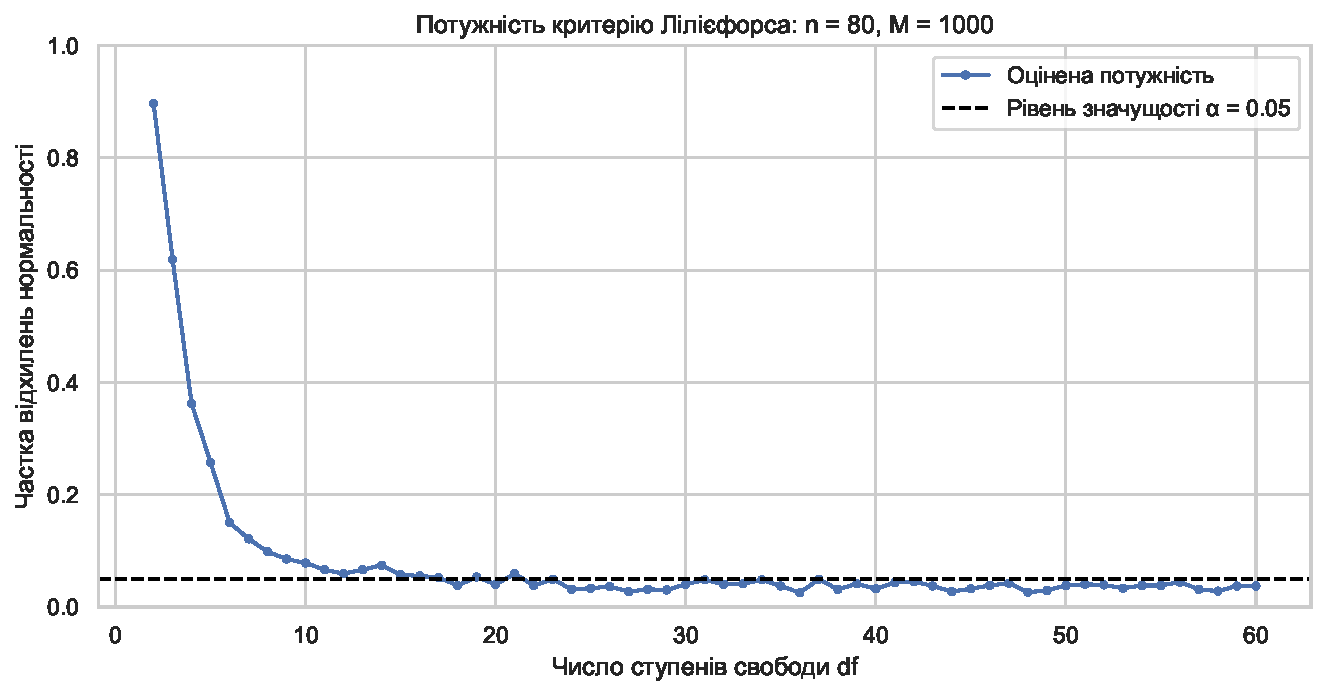
\includegraphics[width=0.90\linewidth]{../figures/part5_power.pdf}
\caption{Емпірична потужність проти t-альтернатив: усі ступені свободи від 2 до 60.}
\end{figure}

\subsection*{Повні результати моделювання потужності}
Для кожного значення $df$ виконано 1000 тестів. $R$ - кількість відхилень нормальності, $\widehat\pi=R/1000$ - оцінка потужності.

\begin{table}[H]
\centering
\small
\caption{Результати всіх 59 серій симуляцій.}
\begin{tabular}{rrr@{\qquad}rrr@{\qquad}rrr}
\toprule
$df$ & $R$ & $\widehat\pi$ & $df$ & $R$ & $\widehat\pi$ & $df$ & $R$ & $\widehat\pi$ \\
\midrule
2 & 897 & 0.897 & 22 & 38 & 0.038 & 42 & 45 & 0.045 \\
3 & 619 & 0.619 & 23 & 49 & 0.049 & 43 & 37 & 0.037 \\
4 & 362 & 0.362 & 24 & 31 & 0.031 & 44 & 27 & 0.027 \\
5 & 257 & 0.257 & 25 & 33 & 0.033 & 45 & 32 & 0.032 \\
6 & 150 & 0.150 & 26 & 36 & 0.036 & 46 & 38 & 0.038 \\
7 & 121 & 0.121 & 27 & 27 & 0.027 & 47 & 42 & 0.042 \\
8 & 98 & 0.098 & 28 & 31 & 0.031 & 48 & 26 & 0.026 \\
9 & 85 & 0.085 & 29 & 30 & 0.030 & 49 & 29 & 0.029 \\
10 & 78 & 0.078 & 30 & 40 & 0.040 & 50 & 38 & 0.038 \\
11 & 66 & 0.066 & 31 & 48 & 0.048 & 51 & 40 & 0.040 \\
12 & 59 & 0.059 & 32 & 40 & 0.040 & 52 & 39 & 0.039 \\
13 & 66 & 0.066 & 33 & 41 & 0.041 & 53 & 33 & 0.033 \\
14 & 74 & 0.074 & 34 & 48 & 0.048 & 54 & 38 & 0.038 \\
15 & 57 & 0.057 & 35 & 37 & 0.037 & 55 & 38 & 0.038 \\
16 & 55 & 0.055 & 36 & 25 & 0.025 & 56 & 44 & 0.044 \\
17 & 52 & 0.052 & 37 & 49 & 0.049 & 57 & 31 & 0.031 \\
18 & 38 & 0.038 & 38 & 31 & 0.031 & 58 & 28 & 0.028 \\
19 & 53 & 0.053 & 39 & 41 & 0.041 & 59 & 37 & 0.037 \\
20 & 40 & 0.040 & 40 & 32 & 0.032 & 60 & 37 & 0.037 \\
21 & 59 & 0.059 & 41 & 43 & 0.043 &  &  &  \\
\bottomrule
\end{tabular}
\end{table}

\end{document}
